\documentclass[12pt]{article}
\usepackage{geometry}
\geometry{a4paper, margin=1in}
\usepackage{booktabs}
\usepackage{multirow}
\usepackage{graphicx}

\begin{document}

\title{Part B: Instruction Extension Breakdown}
\author{Syed Faraz \& Ryyan Alvi}
\date{}
\maketitle

\section*{Brainstorming Notes}
\begin{center}
    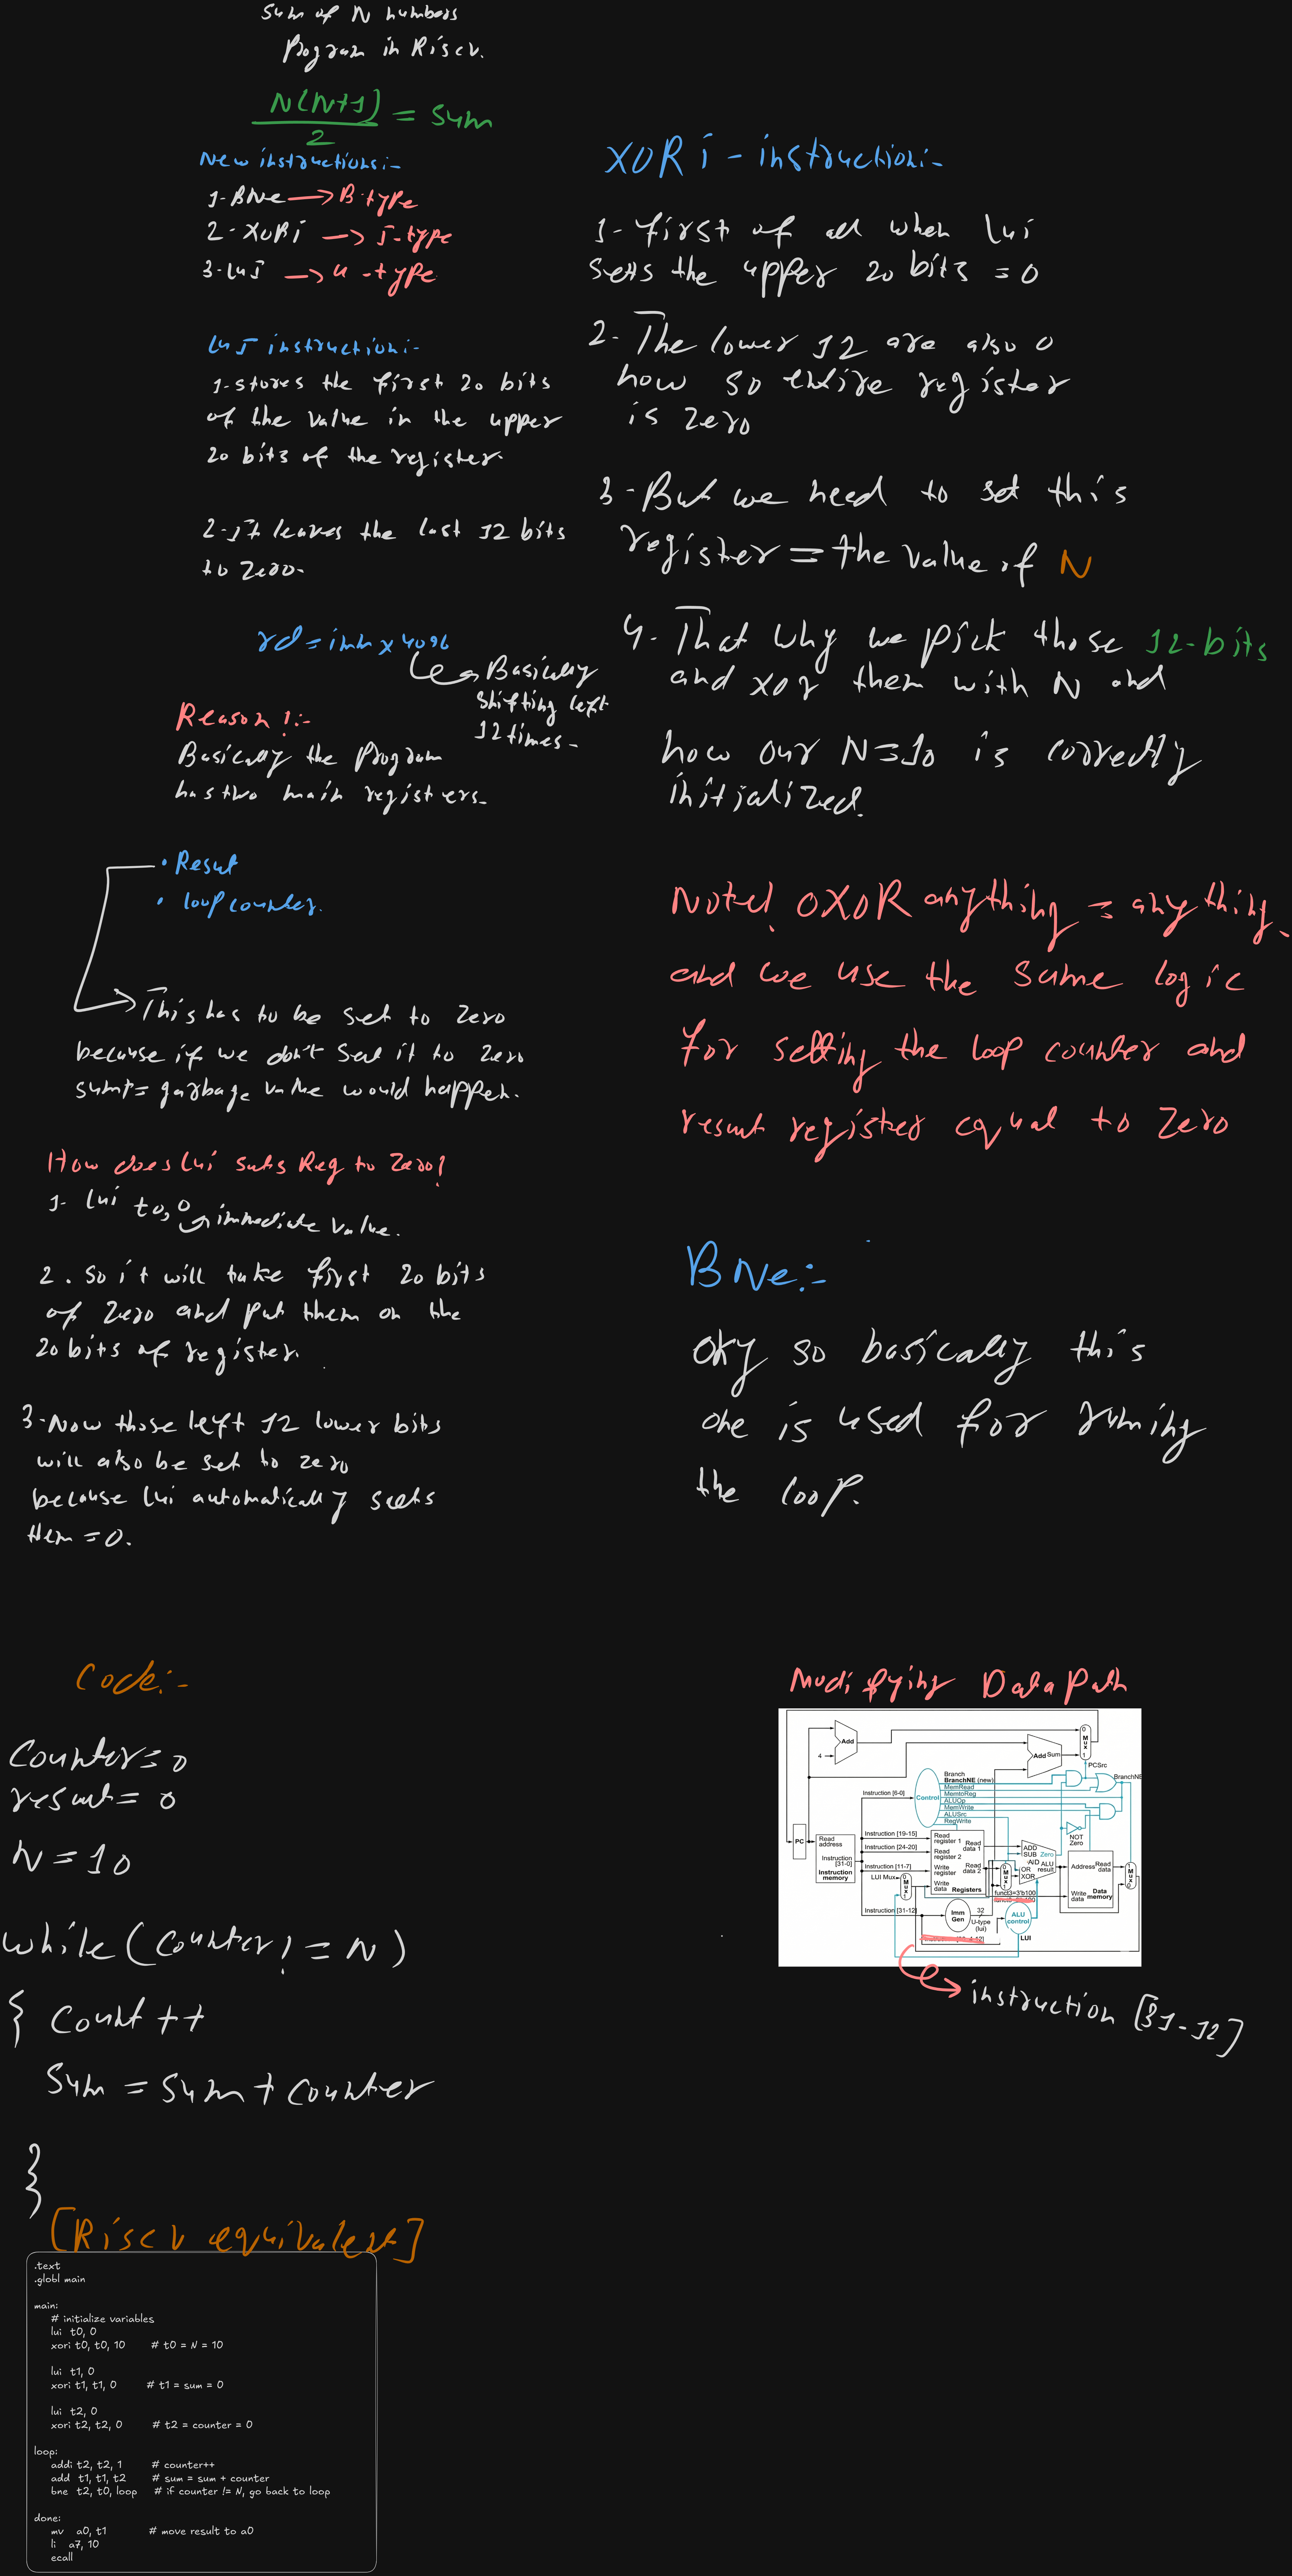
\includegraphics[width=\textwidth,height=0.45\textheight,keepaspectratio]{CA-PROJECT-NOTES.png}
\end{center}

\vspace{0.5cm}

\section*{1. Instruction: LUI (U-Type)}
\textbf{Assembly:} \texttt{lui x1, 0x12345} \\
\textbf{Hex Code:} \texttt{0x123450B7} \\
\textbf{Binary:} \texttt{00010010001101000101000010110111}

\vspace{0.5cm}
\noindent
\begin{tabular}{|c|c|c|}
\hline
\textbf{imm[31:12]} & \textbf{rd} & \textbf{opcode} \\
(20 bits) & (5 bits) & (7 bits) \\
\hline
00010010001101000101 & 00001 & 0110111 \\
\hline
0x12345 & x1 & lui \\
\hline
\end{tabular}

\vspace{1cm}

\section*{2. Instruction: XORI (I-Type)}
\textbf{Assembly:} \texttt{xori x2, x1, 6} \\
\textbf{Hex Code:} \texttt{0x0060C113} \\
\textbf{Binary:} \texttt{00000000011000001100000100010011}

\vspace{0.5cm}
\noindent
\begin{tabular}{|c|c|c|c|c|}
\hline
\textbf{imm[11:0]} & \textbf{rs1} & \textbf{funct3} & \textbf{rd} & \textbf{opcode} \\
(12 bits) & (5 bits) & (3 bits) & (5 bits) & (7 bits) \\
\hline
000000000110 & 00001 & 100 & 00010 & 0010011 \\
\hline
6 & x1 & xor & x2 & OP-IMM \\
\hline
\end{tabular}

\vspace{1cm}

\section*{3. Instruction: BNE (B-Type)}
\textbf{Assembly:} \texttt{bne x4, x3, -4} \\
\textbf{Hex Code:} \texttt{0xFE321EE3} \\
\textbf{Binary:} \texttt{11111110001100100001111011100011}

\vspace{0.5cm}
\noindent
\begin{tabular}{|c|c|c|c|c|c|c|c|}
\hline
\textbf{imm[12]} & \textbf{imm[10:5]} & \textbf{rs2} & \textbf{rs1} & \textbf{funct3} & \textbf{imm[4:1]} & \textbf{imm[11]} & \textbf{opcode} \\
(1 bit) & (6 bits) & (5 bits) & (5 bits) & (3 bits) & (4 bits) & (1 bit) & (7 bits) \\
\hline
1 & 111111 & 00011 & 00100 & 001 & 1110 & 1 & 1100011 \\
\hline
\multicolumn{2}{|c|}{\multirow{2}{*}{imm = -4}} & x3 & x4 & bne & \multicolumn{2}{c|}{\multirow{2}{*}{imm = -4}} & BRANCH \\
\cline{3-5}\cline{8-8}
\multicolumn{2}{|c|}{} & \multicolumn{3}{c|}{} & \multicolumn{2}{c|}{} & \\
\hline
\end{tabular}

\vspace{0.5cm}
\textbf{Immediate Calculation for BNE (-4):} \\
Combined bits: \texttt{imm[12|11|10:5|4:1|0]} \\
Result: \texttt{1111111111100} (which is -4 in 13-bit two's complement).

\end{document}
